In the \wh{} analysis, the dominant background in the \zdom{} and \zdep{} SRs arises from $WZ/W\gamma^{*}$ production. Following the strategy used in the Run~2 analysis, three orthogonal $WZ$ CRs are defined to derive normalization factors (NFs) that correct for potential mis-modeling of this background. These CRs use the same selection criteria as the \zdom{} SR, except they require a SFOS lepton pair with an invariant mass within 25~GeV of the $Z$ boson mass. To account for the jet multiplicity dependence observed in Run~2, the control regions are categorized by jet count: a 0-jet CR (WZCR 0j), a 1-jet CR (WZCR 1j), and a 2-or-more jet CR (WZCR 2+j). The normalization factors extracted from these regions are constrained in the statistical analysis described in Chapter~\ref{ch:statistical_analysis}. Figure~\ref{fig:vh_wh_wzcr_numjets} show the pre-fit MC/data agreement in each $WZ$ CR, where potential mis-modeling of the background is observed.

\begin{figure}[htp]
  \centering
  \subfloat[$WZ$ 0-jet CR]{
    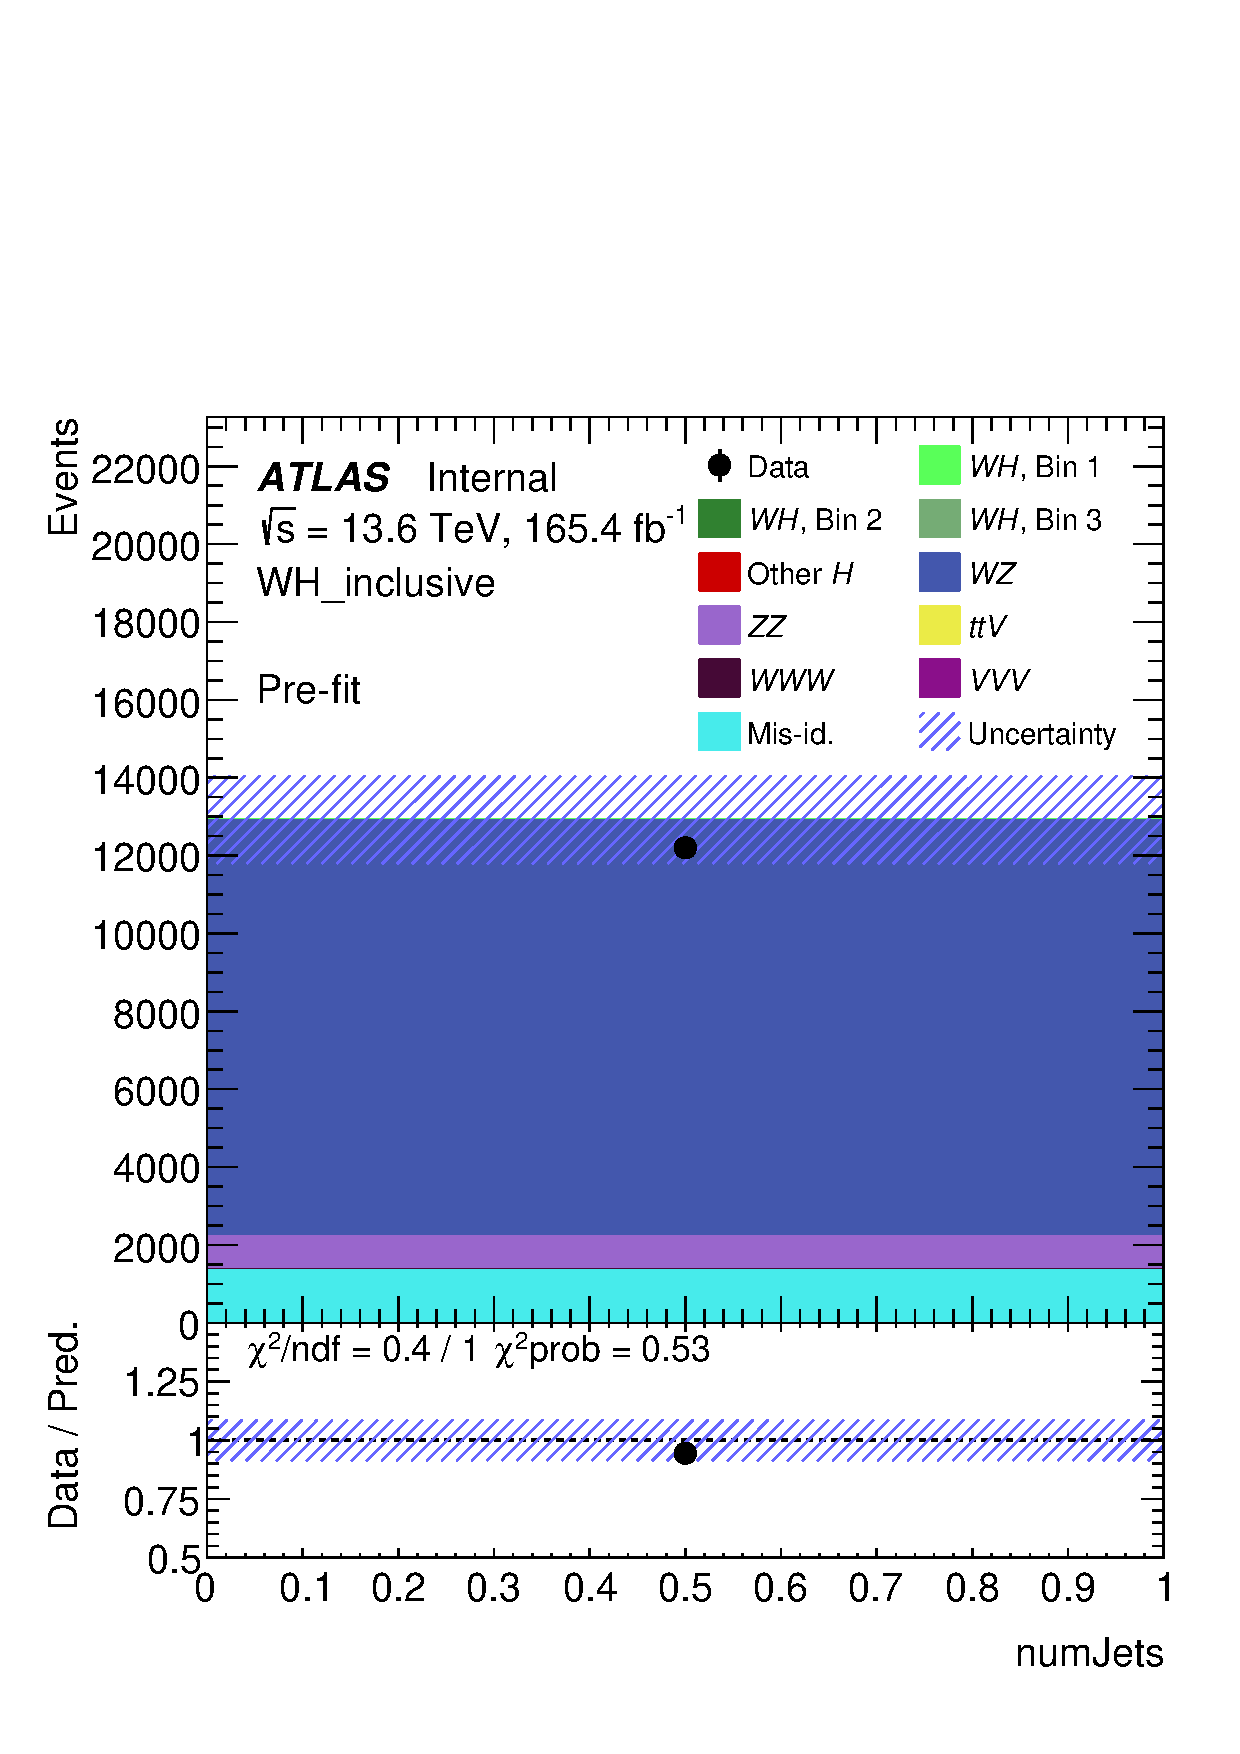
\includegraphics[width=0.45\textwidth]{figures/VH/VH_wzcr_0jet_numjets.pdf}\label{fig:vh_wh_wzcr_0j_numjets}
  }
  \subfloat[$WZ$ 1-jet CR]{
    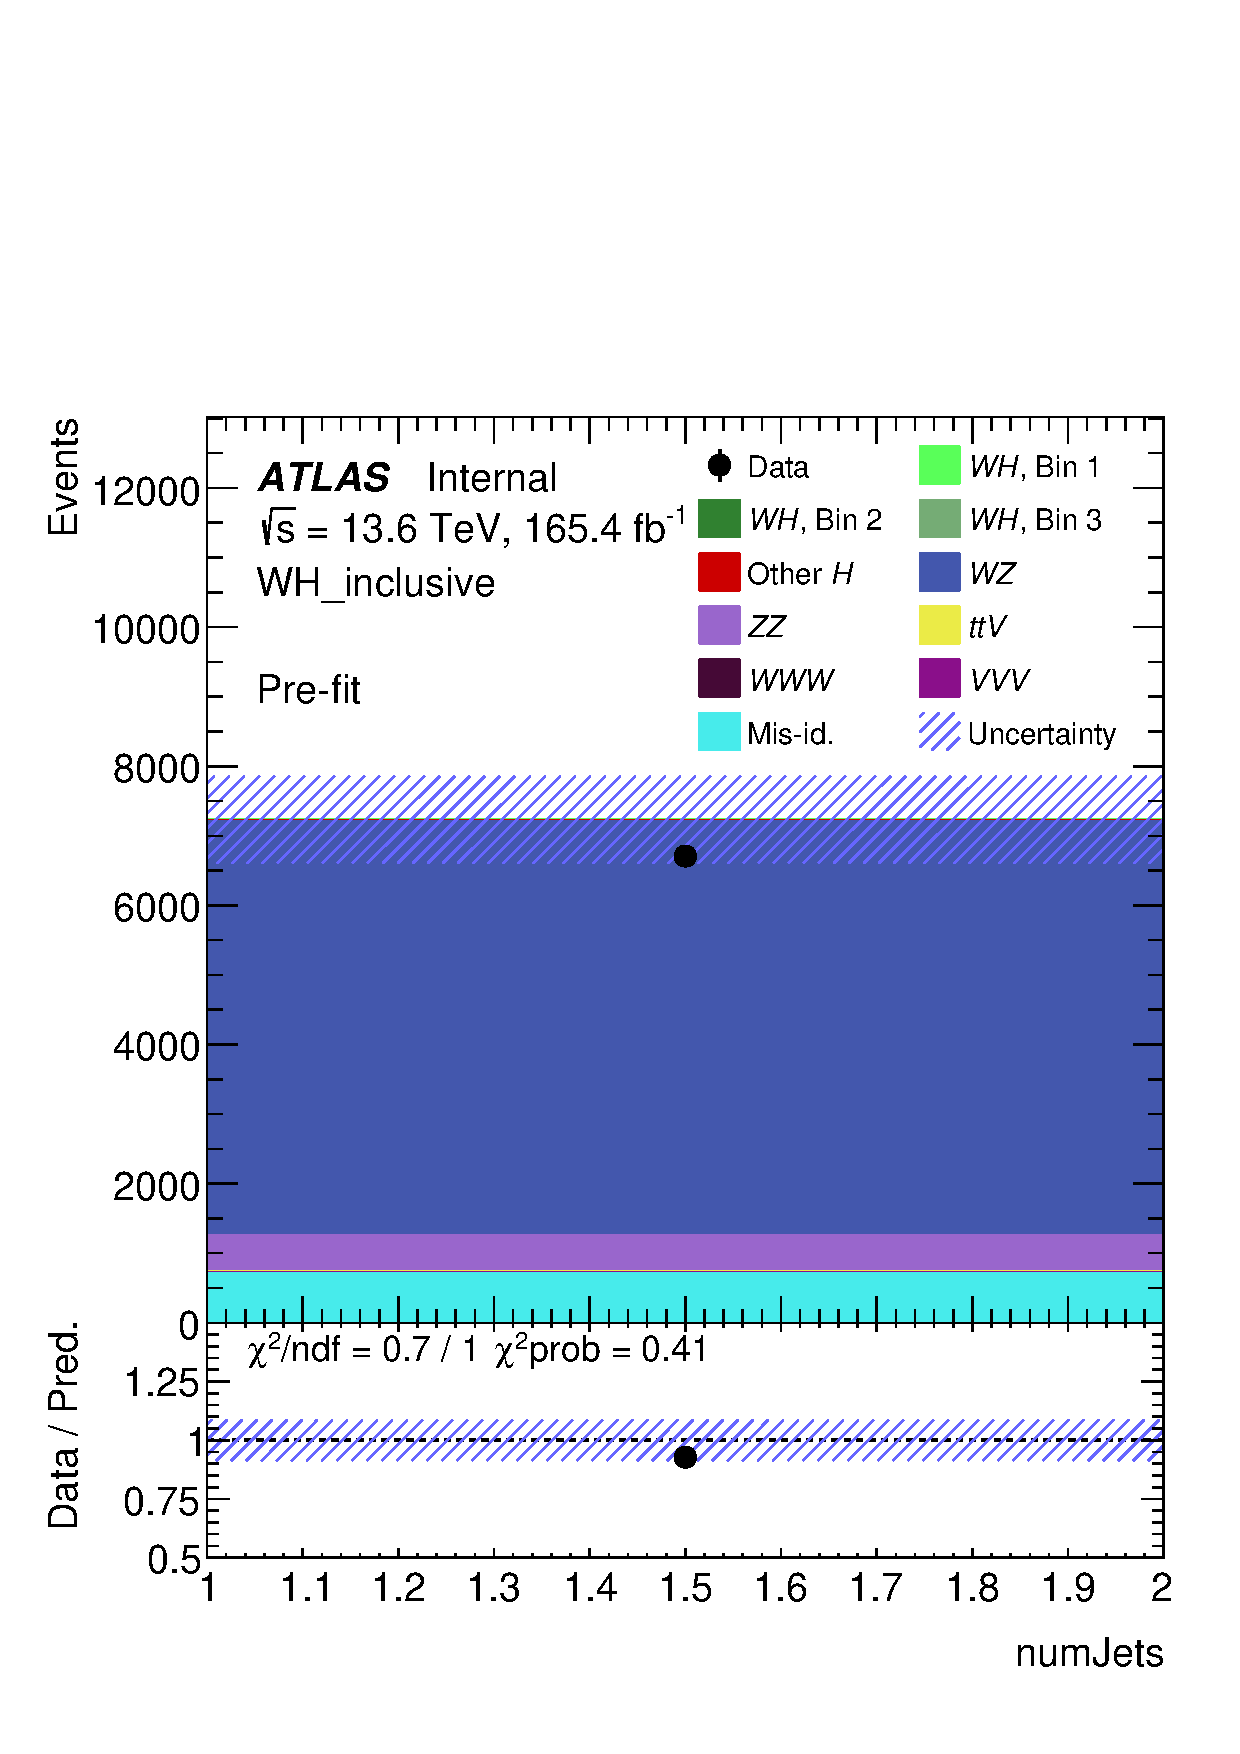
\includegraphics[width=0.45\textwidth]{figures/VH/VH_wzcr_1jet_numjets.pdf}\label{fig:vh_wh_wzcr_1j_numjets}
  }
  \hfill
  \subfloat[$WZ$ 2-or-more jet CR]{
    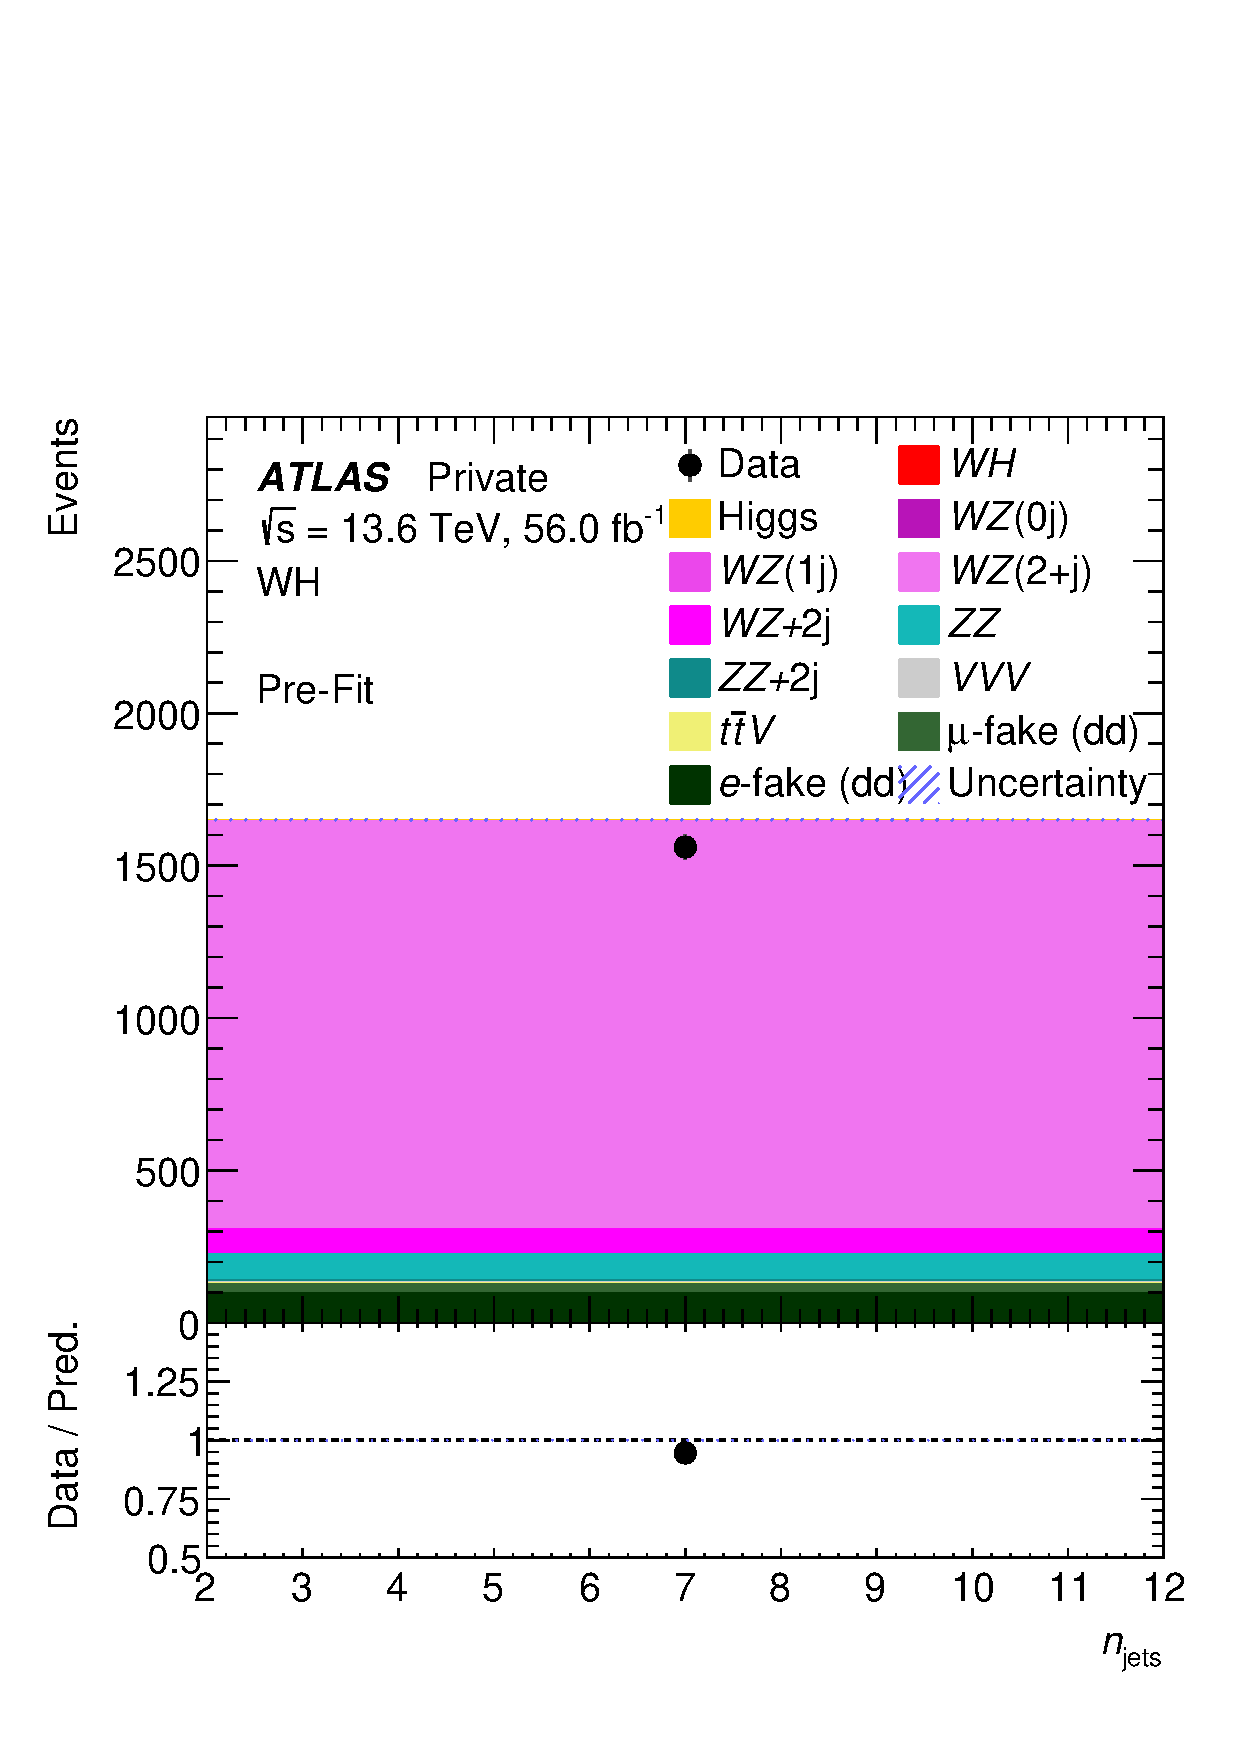
\includegraphics[width=0.45\textwidth]{figures/VH/VH_wzcr_2jet_numjets.pdf}\label{fig:vh_wh_wzcr_2j_numjets}
  }
  \caption{Pre-fit MC/data agreement in the $WZ$ CRs. The $WZ$ 0-jet CR is shown in (a), the $WZ$ 1-jet CR in (b), and the $WZ$ 2-or-more jet CR in (c).}\label{fig:vh_wh_wzcr_numjets}
\end{figure}